% !TEX root = ../../main.tex
\subsection*{Biological sliding-window rerun}

The biological examples use the Tree-of-Life panels from the original SatuTe paper. The protein analysis uses the ribosomal-protein 2D tree, and the nucleotide analysis uses the 16S rRNA 3D tree. In both trees, the highlighted internal split is the branch leading to Eukaryota. The yeast branch is an external branch within the Eukaryota subtree and is the second focal branch in the sliding-window analyses.

\begin{figure}[!p]
  \vspace*{-2.2cm}
  \centering
  \makebox[\textwidth][c]{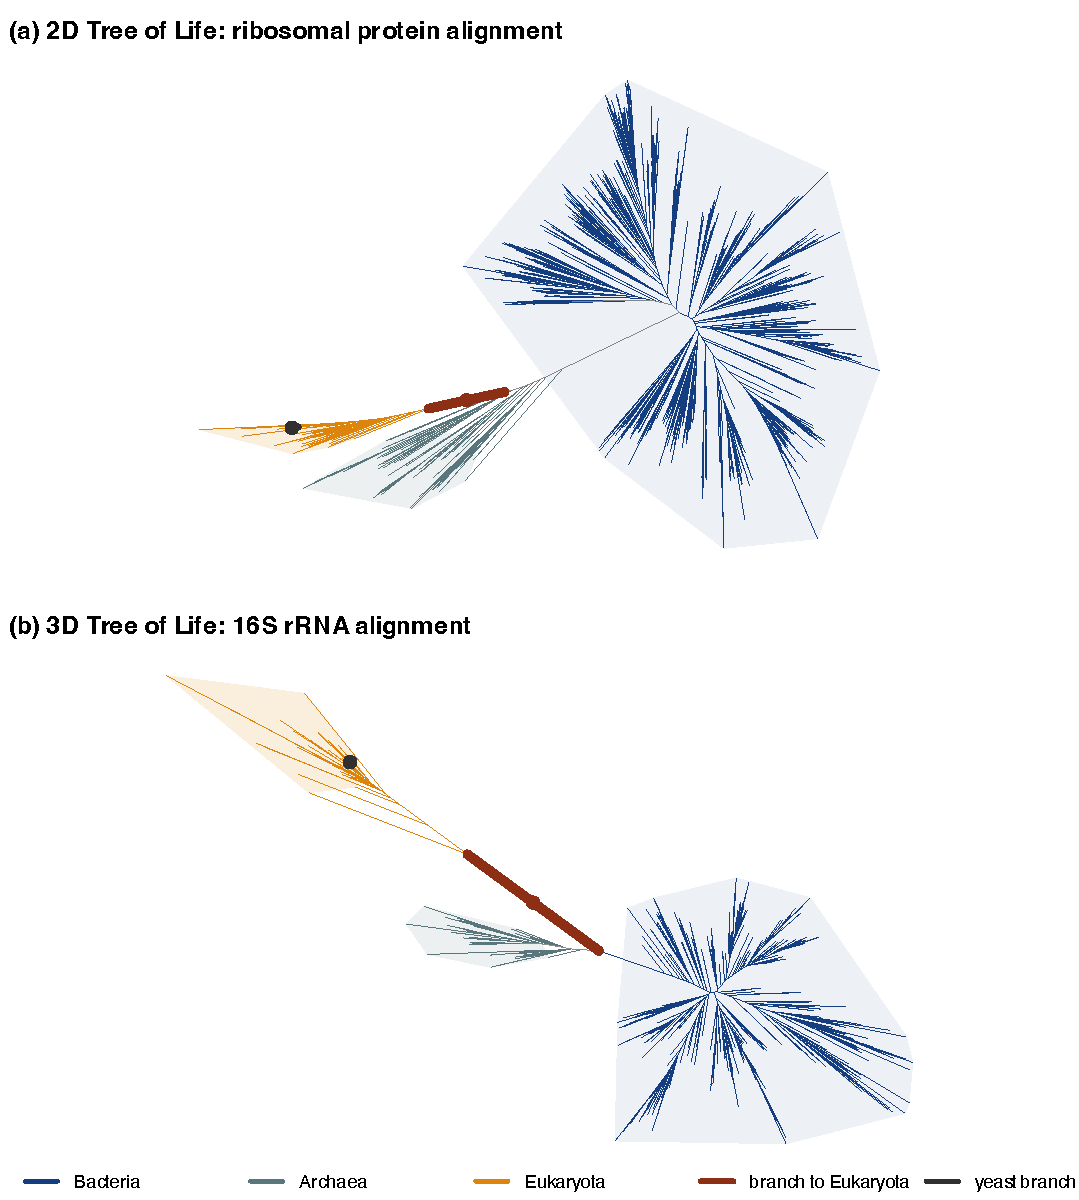
\includegraphics[width=1.06\textwidth]{figures/figure_tree_of_life_reference.pdf}}
  \caption{\textbf{Tree-of-Life references for the biological reruns.} \textbf{a,} Ribosomal-protein 2D tree. \textbf{b,} 16S rRNA 3D tree. Branch colors and translucent hulls identify Bacteria, Archaea and Eukaryota. The highlighted internal segment marks the branch leading to Eukaryota, and the black marker identifies the yeast branch used as the external-branch reference.}
\end{figure}

The curated biological rerun applies the same comparison to the 16S rRNA Tree-of-Life dataset shown in the 3D tree panel. The dataset has \(1{,}947\) alignment sites, a fitted GTR+F+G4 model, four rate categories and 36-site sliding windows. The comparison includes the published SatuTe rerun, a native SatuTe recomputation using \(C_{\partial 1}\), and a native eigenvalue-weighted recomputation. Differences between the published and native SatuTe curves reflect differences in implementation and input files. The formula comparison is therefore the native SatuTe recomputation versus the native eigenvalue-weighted recomputation.

For the branch leading to Eukaryota, the published SatuTe rerun marks \(822\) of \(1{,}912\) windows as saturated. The native SatuTe recomputation marks \(895\) windows, whereas the native eigenvalue-weighted recomputation marks \(699\) windows. For the yeast branch, the corresponding counts are \(70\), \(83\) and \(29\) saturated windows. The published-to-native difference is not used as a formula-effect estimate.

A second biological rerun uses an independent implementation that does not read SatuTe component files or SatuTe result trees. It recomputes the sliding-window scores from the IQ-TREE treefile, model report, site-probability output and original alignments for both Tree-of-Life examples \cite{minh2020iqtree}. The z-score curves show the same branch order and window size as the published sliding-window analysis. Because this rerun contrasts published outputs with an independent recomputation, the curves are not used as the primary formula-effect estimate.

\begin{figure}[p]
  \centering
  
\includegraphics[width=0.98\textwidth]{figures/published_vs_eigenvalue_weighted_curves.pdf}
  \caption{\textbf{Published SatuTe and independent eigenvalue-weighted sliding-window curves in the Tree-of-Life examples.} Curves show 36-site window \(Z\)-scores for the branch leading to Eukaryota and for the yeast branch in the ribosomal-protein 2D tree and the 16S rRNA 3D tree. The dashed line marks \(z_\alpha\).}
\end{figure}

In the protein 2D tree, the branch leading to Eukaryota has \(2{,}561\) windows. The saturated-window counts are \(138\) in the published SatuTe rerun and \(5\) in the native eigenvalue-weighted recomputation. The yeast branch also has \(2{,}561\) windows, with counts \(54\) and \(8\). In the 16S rRNA 3D tree, the branch leading to Eukaryota has \(1{,}912\) windows, with counts \(822\) and \(699\). The yeast branch has \(1{,}912\) windows, with counts \(70\) and \(29\). These counts summarize the threshold crossings in the sliding-window curves.

\begin{figure}[htbp]
  \centering
  
\includegraphics[width=0.98\textwidth]{figures/published_vs_eigenvalue_weighted_saturated_windows.pdf}
  \caption{\textbf{Published SatuTe and independent eigenvalue-weighted sliding-window calls in the Tree-of-Life examples.} Bars show the fraction of windows classified as saturated for the branch leading to Eukaryota and for the yeast branch. Numbers above bars give saturated-window counts.}
\end{figure}
\clearpage
